%; whizzy chapter
% -initex iniptex -latex platex -format platex -bibtex jbibtex -fmt fmt
% 以上 whizzytex を使用する場合の設定。

%     Tokyo Debian Meeting resources
%     Copyright (C) 2010 Junichi Uekawa
%     Copyright (C) 2010 Nobuhiro Iwamatsu

%     This program is free software; you can redistribute it and/or modify
%     it under the terms of the GNU General Public License as published by
%     the Free Software Foundation; either version 2 of the License, or
%     (at your option) any later version.

%     This program is distributed in the hope that it will be useful,
%     but WITHOUT ANY WARRANTY; without even the implied warranty of
%     MERCHANTABILITY or FITNESS FOR A PARTICULAR PURPOSE.  See the
%     GNU General Public License for more details.

%     You should have received a copy of the GNU General Public License
%     along with this program; if not, write to the Free Software
%     Foundation, Inc., 51 Franklin St, Fifth Floor, Boston, MA  02110-1301 USA

%  preview (shell-command (concat "evince " (replace-regexp-in-string "tex$" "pdf"(buffer-file-name)) "&"))
% 画像ファイルを処理するためにはebbを利用してboundingboxを作成。
%(shell-command "cd image201005; ebb *.png")

%%ここからヘッダ開始。

\documentclass[mingoth,a4paper]{jsarticle}
\usepackage{monthlyreport}

% 日付を定義する、毎月変わります。
\newcommand{\debmtgyear}{2010}
\newcommand{\debmtgmonth}{5}
\newcommand{\debmtgdate}{17}
\newcommand{\debmtgnumber}{64}

\begin{document}

\begin{titlepage}
\thispagestyle{empty}

% タイトルページ:編集必要な部分は最初のマクロに飛ばすこと

\vspace*{-2cm}
第\debmtgnumber{}回 東京エリア Debian 勉強会資料\\
\hspace*{-2cm}
\includegraphics[width=210mm]{image201003/debsen.eps}\\
\hfill{}\debmtgyear{}年\debmtgmonth{}月\debmtgdate{}日

% ここはアップデートすること
\rotatebox{10}{\fontsize{32}{32} {\gt 特集1: DebianでのLinuxカーネルと
 の付き合い方}}

\vspace*{-2cm}
\hfill{}
\includegraphics[height=6cm]{image200502/openlogo-nd.eps}
\end{titlepage}

\dancersection{Introduction}{上川 純一}

\begin{multicols}{2}
 
 
 今月のDebian勉強会へようこそ。これからDebianの世界にあしを踏み入れると
 いう方も、すでにどっぷりとつかっているという方も、月に一回Debianについ
 て語りませんか?

 Debian勉強会の目的は下記です。

 \begin{itemize}
 \item \underline{Debian Developer} (開発者)の育成。
 \item 日本語での「\underline{開発に関する情報}」を整理してまとめ、アップデートする。
 \item \underline{場}の提供。
 \begin{itemize}
  \item 普段ばらばらな場所にいる人々が face-to-face で出会える場を提供
	する。
  \item Debian のためになることを語る場を提供する。
  \item Debianについて語る場を提供する。
 \end{itemize}
 \end{itemize}		

 Debianの勉強会ということで究極的には参加者全員がDebian Packageをがりがり
 と作るスーパーハッカーになった姿を妄想しています。情報の共有・活用を通し
 て Debianの今後の能動的な展開への土台として、「場」としての空間を提供す
 るのが目的です。

\end{multicols}

\newpage

\begin{minipage}[b]{0.2\hsize}
 \definecolor{titleback}{gray}{0.9}
 \colorbox{titleback}{\rotatebox{90}{\fontsize{80}{80} {\gt デビアン勉強会} }}
\end{minipage}
\begin{minipage}[b]{0.8\hsize}
\hrule
\vspace{2mm}
\hrule
\tableofcontents
\vspace{2mm}
\hrule
\end{minipage}

\dancersection{事前課題}{上川 純一}

今回の事前課題は以下です:

\begin{enumerate}
 \item 普段使っているLinuxディストリビューションと使ってみたいLinuxディ
       ストリビューションは何ですか?使っている理由、魅力、不満点、使っ
       てみたい理由を教えてください。
\end{enumerate}

この課題に対して提出いただいた内容は以下です。


\begin{prework}{ $BOBED7r(B }

$BIaCJ;H$C$F$$$k(BLinux$B%G%#%9%H%j%S%e!<%7%g%s!'(BDebian /GNU Linux
$B;H$C$F$_$?$$(BLinux$B%G%#%9%H%j%S%e!<%7%g%s!'FC$K$J$7(B
$B;H$C$F$$$kM}M3!'%Q%C%1!<%84IM}$,3Z(B
$BL%NO!'%Q%C%1!<%84IM}$,3Z(B
$BITK~!'FC$K$J$7(B


\end{prework}



\begin{prework}{ $BF#BtM}Ao(B(risou) }

$BIaCJ;H$C$F$$$k%G%#%9%H%j%S%e!<%7%g%s$O(BDebian$B$H(BRedHat$B!#(B
RedHat$B$O;E;v$G$7$+;H$C$F$^$;$s!#(BDebian$B$r;H$C$F$kM}M3$OBg3X;~Be$K=jB0$7$F$$$?8&5f<<$N%5!<%P$,(BDebian$B$@$C$?$+$i!#B>$N%G%#%9%H%j%S%e!<%7%g%s$K?($l$k5!2q$b$"$C$?$1$l$I!"7k6I0lHV;H$$$J$l$?$b$N$r$:$C$H;H$C$F$$$k46$8$G$9!#;H$C$F$_$?$$%G%#%9%H%j%S%e!<%7%g%s$O!"(BUbuntu$B$d(BGentoo$B$J$I!#:#$^$G;H$&5!2q$,$J$+$C$?$N$G!"0lEY;H$C$F$_$?$$!"$H$$$&4JC1$JF05!$G$9!#(B

\end{prework}



\begin{prework}{ $B5HLn(B(yy\_y\_ja\_jp) }

$BIaCJ(B Debian $B$r;H$C$F$$$^$9!%?'!9$J0UL#$G<+M3$@$+$i$G$9!%ITK~$O$"$^$j46$8$F$^$;$s!%(BUbuntu $B$5$s$O$h$j(B global $B$J(B Debian $B$K$b$C$H@.2L$r4T85$7$F$$$?$@$1$k$H$&$l$7$/;W$$$^$9!%(B

\end{prework}



\begin{prework}{ $B868}=(9/(B }

debian
$B7Z$$(B

$B8D?ME*$K$O(Bubuntu$B$G$9$,(B
$B2q<R$,(Bred hat$B$r;HMQ$7$F$$$k$N$G(Bred hat$B$K$b6=L#$,$"$j$^$9!#(B

\end{prework}



\begin{prework}{ hard2259 }

$BIaCJ;H$C$F$$$k(BLinux$B%G%#%9%H%j%S%e!<%7%g%s(B
\begin{itemize}
\item VineLinux
\item Ubuntu
\item CentOS
\end{itemize}

$B;H$C$F$$$kM}M3(B

\begin{itemize}
\item Vine\\
$B!!"13X9;$N<x6H$G;XDj$5$l$F$k$+$i!#(B\\
  $B"1$$$$0UL#$G8O$l$?5;=Q$H$$$o$l$?$b$N$rB?$/;H$C$F$$$k$?$a!"(BLinux$B7O$r0l$+$iJY6/$9$k$K$O$b$C$F$3$$$N%b%N$i$7$$$N$G!#(B\\

\item Ubuntu \\
$B!!"1%<%_<<$N@hGZ$+$i4+$a$i$l$?(B
$B!!"1(BWindows$B$K6a$$%b%N$,$"$k$+$i(B

\item CentOS \\
$B!!"1%<%_<<$N%5!<%P$N(BOS$B$,(BCentOS$B$@$+$i;H$o$6$k$rF@$J$$!#(BRedHat$B7O$N9=B$$H;w$F$$$k$+$i!"2q<R$O$$$C$?$H$-LrN)$D$+$b!#(B
$B"(ITK~$r8@$($k$[$I;H$$9~$s$G$^$;$s$4$a$s$J$5$$!#(B
\end{itemize}


$B;H$C$F$_$?$$(BLinux$B%G%#%9%H%j%S%e!<%7%g%s(B\\
$B!&(BGentoo

$B;H$C$F$_$?$$M}M3(B\\
$B!&(BGentoo\\
$B!!"1?'!9Fq$7$$$H$$$o$l$F$$$k$+$iD)@o$7$F$_$?$$!#(B

\end{prework}



\begin{prework}{ $B%-%?%O%i(B }

$BIaCJ;H$C$F$$$k(BLinux$B%G%#%9%H%j%S%e!<%7%g%s(B:debian, Ubuntu
$B!!!!L5NA$G;H$($k!"%i%$%;%s%94IM}$GG:$^$J$/$FNI$$!"2?$+;H$$$?$$%=%U%H$,(B
$B$"$k$H!V(Bapt-get$B!W$G$9$0;n$;$k!#!!$G$b!"4D6-$K$h$C$F2;$,=P$J$+$C$?$j!"(B
$B%0%i%U%#%C%/$d%W%j%s%?$N%I%i%$%P$GG:$s$@$j!"(BWindows$B0MB8$N(BWeb$B%Z!<%8$K(B
$B%"%/%;%9$G$-$J$+$C$?$j!"?M$K4+$a$k$K$O>/!9G:$^$7$$=j$,$"$k!#(B

$B;H$C$F$_$?$$(BLinux$B%G%#%9%H%j%S%e!<%7%g%s(B:Ubuntu(ARM), Android(?)
$B!!!!%b%P%$%kMQES$GMxMQ$7$F$$$k!V(BZaurus$B!W$N@=IJ<wL?$,$D$-$F$$$k$N$G!"(B
$B$=$N8e7Q$H$7$F!V(BNetWalker$B!W$+!V(BJN-DK01$B!W$H$+!V(BIS01$B!W$N(BAndroid$B5!$,(B
$BM_$7$$$J$!!<$H!";W$C$F$^$7$F!&!&!&!#(B


\end{prework}



\begin{prework}{ KIM\_TPDN }

$B%G%9%/%H%C%WMQES$G(BopenSUSE$B!"(BVPS$B$G(BCentOS$B$r;H$C$F$$$^$9!#$A$J$_$K<+Bp;*$O(BFreeBSD$B$r;HMQ$7$F$$$^$9!#(B

$B;H$C$F$$$kM}M3(B
openSUSE
$B!&(BYaST$B$,$+$J$jJXMx!#(B
$B!&(BKDE$B$,9%$-!#(B

CentOS
$B!&=i$a$F;H$C$?%G%#%9%H%m$@$+$i!#0lDL$j$N$3$H$r$3$l$G3X=,$7$?!#(B
$B!&(BVPS$B$d@l;*$N(BOS$BA*Br;h$K$O$?$$$F$$F~$C$F$k!#(B

$B;H$C$F$_$?$$%G%#%9%H%j%S%e!<%7%g%s(B
$B!&(BArudius
$B!&(BUbuntu Studio



\end{prework}



\begin{prework}{ $B>e@n=c0l(B }

$B$$$^$U$H?6$jJV$k$HIaCJ$b$C$H$b;H$C$F$$$k(B Linux $B%G%#%9%H%j%S%e!<%7%g%s$O(B Android $B$G$9!#(B
$B7HBSEEOC$K%W%j%$%s%9%H!<%k$5$l$F$$$k$N$G;H$$E]$7$F$$$^$9!#(B
$BITK~E@$O%+!<%M%k$r$$$8$l$J$$$3$H$H!"(Bemacs$B$,F0$+$J$$$3$H$G$9!#(B


\end{prework}



\begin{prework}{ compozz }

$B!&IaCJ;H$C$F$$$k%G%#%9%H%j%S%e!<%7%g%s(B
$B!!(BUbuntu
$B!&;H$C$F$_$?$$%G%#%9%H%j%S%e!<%7%g%s(B
$B!!(BFedora

$B!&(B(Ubuntu$B$r(B)$B;H$C$F$$$kM}M3(B
$B!!%f!<%6!<$NB?$5$d0BDj@-$,$"$k!J$H;W$C$F$$$k!K$+$i$G$9!#(B

$B!&L%NO(B
$B!!(BKNOOPIX$B$N(BLiveCD$B$r;H$*$&$H$7$?;~!"5/F0;~$+$i%G%#%9%W%l%$%I%i%$%P$G$O$^$C$?$1$l$I!"(BUbuntu$B$O@_DjJQ99$7$J$/$F$b%$%s%9%H!<%k2hLL$+$i(BGUI$B$G46F0$7$^$7$?!#(B
$B!!$H$K$+$/(BLinux$B$NCf$G$OF3F~$d1?MQ$,3Z$@$H;W$&$N$G!"IaCJ;H$$$K$H$F$bLrN)$C$F$$$^$9!#(B

$B!&ITK~E@(B
$B!!%G%#%9%H%j%S%e!<%7%g%s$NITK~$O$[$H$s$IL5$$$G$9$,!"5M$^$C$?$H$-$K(BUbuntu$B$N%P%0$@$C$?$j$7$F$,$C$+$j$7$?$3$H$,$"$j$^$9!#(B

$B!&(B(Fedora$B$r(B)$B;H$C$F$_$?$$M}M3(B
$B!!;H$C$F$_$?$3$H$,$J$$$+$i$G$9!#(B Gentoo$B$O;~4V$,$"$l$P!#(B
Debian$BJY6/2q$J$N$K$9$_$^$;$s!#!#!#(B

\end{prework}



\begin{prework}{ mnakao }

$BIaCJ;H$C$F$$$k(BLinux$B%G%#%9%H%j%S%e!<%7%g%s!'(B
$B$=$l$O(BDebian$B$G$7$g$&!*(B

$B;H$C$F$_$?$$(BLinux$B%G%#%9%H%j%S%e!<%7%g%s!'(B
openSUSE$B$r;E;v$G>/$7;H$C$F$_$?$1$I!"7k9=JXMx$=$&$J$N$G5$$K$J$C$F$^$9!#(B

$B!J(BDebian$B$r!K;H$C$F$$$kM}M3!"L%NO!'(B
apt$B$,JXMx$J$N$H!"0lEY%$%s%9%H!<%k$7$?$i!":F%$%s%9%H!<%k$9$kI,MW$,$J$$$3$H!J;d$O%X%?%l$J$N$G!"2?EY$b%/%j!<%s%$%s%9%H!<%k$7$F$^$9$,(B:p$B!K(B

$B!J(BDebian$B$N!KITK~E@!'(B
$BF~Lg<T$O$=$NJ82=$K47$l$k$N$,BgJQ$J=j!#(B

$B!J(BSuse$B$r!K;H$C$F$_$?$$M}M3!'(B
YaST$B$,$"$k$+$i!#(BLDAP$B$N@_Dj$b(BYaST$B$G=PMh$k$N$GJXMx$=$&!#(B


\end{prework}



\begin{prework}{ koedoyoshida }

$BIaCJ;H$C$F$$$k(BLinux$B%G%#%9%H%j%S%e!<%7%g%s(B
Debian,Ubuntu,Asianux,RHEL
$B;H$C$F$_$?$$(BLinux$B%G%#%9%H%j%S%e!<%7%g%s$O2?$G$9$+!)(B
Gentoo
$B;H$C$F$$$kM}M3(B
Debian:$B%Q%C%1!<%8$,B?$$!#(Bstable$B$N%P!<%8%g%s%"%C%W$,CY$$$N$G!"%5!<%P8~$1$K0BDj$7$F$$$k!#%$%s%9%H!<%k8e$N<j4V$,3]$+$i$J$$!#(B
Ubuntu:$B%Q%C%1!<%8$,B?$$!#%+!<%M%k$,?7$7$/!"(BLiveCD$B$,I8=`$J$N$G?77?5!$G3F<o%G%P%$%9$NF0:n$r3NG'$9$k$N$KJXMx!#%$%s%9%H!<%k$N<j4V$,3]$+$i$J$$!#(B
Asianux:$BHS$N<o(B
RHEL:$BNI$/$b0-$/$bI8=`$G;29M$K$J$k(B
$BL%NO!"ITK~E@!";H$C$F$_$?$$M}M3(B
Gentoo:$B%Q%C%1!<%8$NB?$5!"<j4V$,$+$+$j$=$&$J$H$3$m!"%^%K%"8~$1(B


\end{prework}



\begin{prework}{ moli3 }

$BIaCJ;H$C$F$$$k%G%#%9%H%j%S%e!<%7%g%s(B
CentOS
$BN>J}=i?4<T$K$O$J$+$J$+Fq$7$$$h$/m5$/$3$H$,$"$j$^$9!#(B
$B%5!<%P$K8~$$$F$$$k$HJ9$$$F%5!<%P$H$7$F;H$C$F$$$^$7$?!#(B
Debian
$B:G6a%5!<%P$H%G%#%9%/%H%C%W$r%5!<%P$K$7$^$7$?!#(BCentOS$B$H0c$&E@$G(B
$B8MOG$&$H$-$,$"$j$^$9!#(B
$B;H$C$F$_$?$$%G%#%9%H%j%S%e!<%7%g%s(B
gentoo
$B$h$/$o$+$i$J$$$1$IOCBj$J$N$GF~$l$F$_$?$$$G$9!#(BDebian$B$+$i(Bchroot$B$G(B
$B$d$m$&$+$H;W$C$F$^$9!#(B

\end{prework}



\begin{prework}{ $BB<ED?.?M(B }

$B;H$C$F$$$k(B: Ubuntu
+ $BH>G/$4$H$K40@.EY$N9b$$%P!<%8%g%s$,%j%j!<%9$5$l$k$H$$$&%5%$%/%k(B
+ Humanity$B%"%$%3%s%F!<%^(B
+ Mark Shuttleworth$B$N9TF0NO(B
- Mark Shuttleworth$B$N9TF0NO(B

$B;H$C$F$_$?$$(B: Debian
stable, testing, unstable$B$rJBNs$G?J$a$F$$$k$H$3$m!#(B

\end{prework}



\begin{prework}{ akedon }

$BIaCJ;H$C$F$$$k(BLinux$B%G%#%9%H%j%S%e!<%7%g%s$O(BDebian,CentOS,MIKO GNYO/Linux (Ubuntu Desktop) $B$G$9!#(B
$B;H$C$F$_$?$$(BLinux$B%G%#%9%H%j%S%e!<%7%g%s$O(BSuSE$B$G$9$M!#(B
$BA05-$N(BLinux$B$r;H$C$F$$$kM}M3$O(BDebian$B$O;H$$;O$a$?Ev;~$O05E]E*$K(Bapt$B%D!<%k$,B>$N4IM}%D!<%k(Brpm$B$h$j;H$$$d$9$+$C$?$N$G!"$=$3$+$i;H$$B3$1$F47$l$F$$$k$+$i$G$9!#(BCentOS$B$O(BXen$B$r;H$$;O$a$?;~$K0lHV<j7Z$G3N<B$KF0$$$?$+$i$G$9!#(BMIKO GNYO/Linux$B$OJI;f$,AGE($G$9$h$M!"Mn$ACe$$$F:n6H$9$k$K$O:GE,$G$9!#(B 
$BL%NO$O(BLinux$BA4BN$K8@$($k$3$H$G$9$,!"ITMW$J5!G=$r;_$a$?$j:o=|$7$?$j!"I,MW:GDc8B$K9J$j9~$_$d$9$/!";H$$$d$9$$MM$K%+%9%?%^%$%:$7$d$9$$$H$$$&E@$K$"$j$^$9!#(B
$BITK~E@$O!"%G%P%$%9%I%i%$%PEy!"%Y%s%@$K0MB8$7$F$$$k$b$N$,(BWindows$B$d(BMacOS$B$K8+Nt$j$9$k$b$N$,$"$C$?$j$9$kE@$K$J$j$^$9!#(B
SuSE$B$r;H$C$F$_$?$$M}M3$OC1=c$G!"L$$@;n$7$F$$$J$$$+$i$G$9!#(B

\end{prework}



\begin{prework}{ yama1066 }

$BIaCJ;H$C$F$$$k(BLinux$B%G%#%9%H%j%S%e!<%7%g%s!'(B
Debian GNU/Linux (sid, squeeze on lenny)
$B;H$C$F$$$kM}M3!'$J$s$H$J$/!#(B
$BL%NO!'$J$K$+$"$C$?$+$J!)!J$*(B
$BITK~E@!'FC$KL5$7!#(B

$BIaCJ;H$C$F$O$$$J$$$,!"(Bapt-get upgrade $B$@$1$7$F$$$k(BLinux$B%G%#%9%H%j%S%e!<%7%g%s!'(B
Ubuntu Linux (maverick)
$B;H$C$F$$$kM}M3!';H$C$F$J$$!#(B
$BL%NO!'(BDebian$B>e$G$b(B chroot $B$G6&B82DG=!#(B
$BITK~E@!'FC$KL5$7!#(B

$B;H$C$F$_$?$$(BLinux$B%G%#%9%H%j%S%e!<%7%g%s!'(BFedora (Rawhide)
$B;H$C$F$_$?$$M}M3!'?MCl$O=EMW$@$h$M!#(B

\end{prework}



\begin{prework}{ $B4d>>(B $B?.MN(B }

$BIaCJ;H$C$F$$$k(BLinux$B%G%#%9%H%j%S%e!<%7%g%s(B
Debian, Gentoo, buildroot, openembedded, $B%*%l%*%l(Bbusybox$B%Y!<%9%G%#%9%H%j(B

$B;H$C$F$_$?$$(BLinux$B%G%#%9%H%j%S%e!<%7%g%s(B
Arch Linux $B$H$+!#$J$s$+?M5$$,$"$k$h$&$G$9!#(B
$B;H$C$F$$$kM}M3!"L%NO!"ITK~E@!";H$C$F$_$?$$M}M3(B
Debian: $B;E;v$H3+H/MQ!#(B
Gentoo: $B3+H/MQ$G<g$K(BGCC$B$N(BHEAD$B$rDI$C$+$1$k$N$K;H$C$F$$$^$9!#(B
buildroot: $B;E;v$G!#%/%m%9%3%s%Q%$%i$H$+0l<0$r$H$j$"$($::n$k>l9g$KMxMQ$7$F$$$^$9!#%G%#%9%H%j$H$$$&$N$+$OITL@!#(B
openembedded: $B:G6a$$$8$j$O$8$a$^$7$?!#(Bsh$B%5%]!<%H$H$+!#(B
$B%*%l%*%l(Bbusybox$B%Y!<%9%G%#%9%H%j(B: 


\end{prework}



\begin{prework}{ monoqlo }

$BIaCJ;H$C$F$$$k(BLnux$B%G%#%9%H%j%S%e!<%7%g%s!'(BUbuntu
$B;H$C$F$_$?$$(BLinux$B%G%#%9%H%j%S%e!<%7%g%s!'$7$P$i$/(BUbuntu$B$G$$$$$G$9!#(B
$B;H$C$F$$$kM}M3!'F|K\8l$N>pJs$,$?$/$5$s$"$k$3$H$H!"=i$a$F(BLinux$B$r;H$*$&$H;W$C$?;~$K(BWindows$B$+$i$N0\9T$,3Z$@$H46$8$?$?$a!#(B
$BL%NO!'=i?4<T$K$b4+$a$d$9$$(B
$BITK~E@!'$H$/$K$J$7(B

\end{prework}



\begin{prework}{ $B$J$+$*$1$$$9$1(B }

$B;H$C$F$$$k%G%#%9%H%j%S%e!<%7%g%s$O(BDebian$B$G!"D94|E*$K;H$($=$&$J$N$,L%NO$G$9!#(B
$B;H$C$F$_$?$$%G%#%9%H%j%S%e!<%7%g%s$O!"(BScientific Linux$B$G$9!#(B

\end{prework}



\begin{prework}{ henrich }

$BIaCJ$O(B debian$B!"$=$N>e$N(B KVM $B$G(B fedora $B$H(B ubuntu $B$,$?$^$KF0$-$^$9!#(B

$B;H$C$F$_$?$$$N$O!D(BCentOS$B$+$J$!!#2?$,NI$$$N$+L%NO$,$h$/J,$+$i$s$N$G!#8eBg85$N(B RHEL$B!#(B2.1 $B$0$i$$$N;~$K%$%s%9%H!<%k$7$?5-21$7$+$J$$$N$G!#(B

\end{prework}



\begin{prework}{ $B$^$($@$3$&$X$$(B }

$BIaCJ;H$C$F$$$k%G%#%9%H%m$O(BDebian$B$G$9!#B>$K;H$C$F$_$?$$$N$OL5$$$G$9!#J#?t<oN`$N%"!<%-%F%/%A%c$GF1$8%7%9%F%`$r;H$($k(B($B%5%]!<%H$7$F$$$k%"!<%-%F%/%A%c$,B?$$(B)$B$N$,0lHV$NM}M3$G$9!#(B($B$$$D$b8@$C$F$$$kM}M3$HF1$8$GBe$o$j1G$($7$^$;$s$,(B)

\end{prework}



\begin{prework}{ $BAR@$8E(B $B63J?(B }

$BIaCJ(B: Fedora 11$B!#E,Ev$KF0$/$N$G!#>pJs$,B?$/$F5M$^$C$F;`$L$3$H$,>/$J$$!#JQ$K$3$@$o$j$r$b$C$F;H$C$F$k?M$,B?$$$N$G$?$^$K5DO@$,$+$_9g$o$J$/$F:$$k(B
$B;H$C$F$_$?$$(B: OpenSUSE$B!#7k9=I_5o$,9b$$$H;W$C$F$$$?$i!":G6a<~0O$G;H$C$F$$$k?M$,A}$($?$N$G!#(B

\end{prework}



\begin{prework}{ $BKYK\(B $B5.9,(B (opentaka) }

$BIaCJ;H$C$F$$$k(BLinux$B%G%#%9%H%j%S%e!<%7%g%s$H;H$C$F$_$?$$(BLinux$B%G%#%9%H%j%S%e!<%7%g%s$O2?$G$9$+!)(B
---
Gentoo Linux$B$r%a%$%s$K!"(BDebian$B$r(Beee pc$B$G;H$C$F$$$k!#(B
LFS(Linux From Scratch)$B$r;H$$$3$J$7$F$_$?$$!#(B
---

$B;H$C$F$$$kM}M3!"L%NO!"ITK~E@!";H$C$F$_$?$$M}M3$r65$($F$/$@$5$$!#(B
---
Gentoo Linux: 
Portage$B$KB?$/$N%Q%C%1!<%8$,$"$k!#(B

$BITK~E@(B: bleeding edge$B$9$.$F!"K\Ev$K(Bbleeding$B$9$k;~$,$"$k!#(B($B2u$l$k(B)
---

---
Debian(debian eee project): 
eeepc$B8~$1$N%G%#%9%H%j%S%e!<%7%g%s$G0lHV4JC1$K%$%s%9%H!<%k$G$-$=$&$@$C$?$+$i!#(B
---

\end{prework}




\dancersection{最近のDebian関連のミーティング報告}{岩松信洋}
\subsection{東京エリアDebian勉強会63回目報告}
% (query-replace-regexp "<.*?>" "")
% (query-replace-regexp "^[	 ]\+" "")

第63回東京エリアDebian勉強会 を行いました。場所は稲城。

稲城といっても最寄り駅は京王稲城ではなく、若葉台というところ。

参加者は原口秀康さん、キタハラさん、やまねさん、山本さん、koedoyoshidaさ
ん、鈴木崇文さん、藤沢理聡さん、村田信人さん、あけどさん、 Hirotaka
Kawataさん、opentakaさん、松澤二郎さん、前田さん、荒木さん、岩松 の16名
でした。

まず私はpiupartsの使い方と内部の動きについて話しました。piupartsは開発者
寄りのツールです。使うとテストが楽ちんになるので、みなさん使いましょう。

次に前田さんがupstartについて話しました。現状では upstart に移行するメリッ
トがないことがわかりました。upstart-nativeさくっとしたいものですね。

そして、山根さんが debtagsについて話ました。debtagsはあまり知られてない
ので、好評だったようです。現状ではタグの付け方などに問題があるのでこれら
を解決する必要がありそうです。

これらが終わったあとに我らがが荒木新会長からありがたいお言葉をいただきま
した。自分も前会長としてやりたかったことを話したのですが、よくよく考えて
みるとなんか違っていて、自分は Debian JP に入ったのならDebian JP ででき
ることを目標にして活動してほしいというのがあったのでした。

案の定時間が余ったので、ネタ帳にに残っていた Debian/SH4進捗報告会と、
Emdebian の現状と Emdebian/Grip について話しました。

勉強会後の宴会は牛角で。1時間半ほど待たされるプレイをしていました。肉は
うまかったです。

\clearpage

\dancersection{DebianでのLinuxカーネルとの付き合い方}{岩松}

\subsection{はじめに}

ここ数年でDebianのLinuxカーネル開発体制やLinuxカーネルに関するツールの使
い方が変わってきました。Debian JP のMLでもたまにLinuxカーネルに関してハ
マっている方おられるようです。
昔と違って最近のユーザはDebianから提供されているカーネルを使う人が多いよ
うで、ネット上でも情報がまとまっていません。
今回は、Debian Linux カーネル開発の背景と、今時のカーネルコンパイル方法に
ついて簡単にまとめました。

\subsection{Debian Linux カーネルの開発状況}
Debian の Linux カーネルは Debian Kernel Team によって開発およびメンテナ
ンスされています。
もちろんDebianでは LinuxカーネルもDebianパッケージとして提供されており、
容易に利用可能です。
チームコアメンバは Bastian Blank, Frederik Schul, Maximilian Attems,
Ben Hutchings で、彼らがが中心になってメンテナンスしています。各々はもち
ろんカーネル開発者です。
彼らだけでは全アーキテクチャの面倒を見きれないので、各アーキテクチャメン
テナとともにカーネルパッケージをメンテナンスしています。
アーキテクチャメンテナはBuilddメンテナや、Debian-instller チーム、eglibc
メンテナなど、カーネルに関係するパッケージをメンテナンスしている約20名の開発者に
よって構成されます。

\begin{figure}[H]
\begin{center}
\includegraphics[width=1.0\hsize]{image201005/debian-kernel-team.eps}
\caption{Debian Linuxカーネルチーム構成図}
\label{fig:debian-kernel-team}
\end{center}
\end{figure}

\subsection{DebianでのLinuxカーネル開発プロセス}
去年の6月頃まではDebianでベースとするLinuxカーネルバージョンは決まっていましたが、
パッケージのリリースサイクルはあまり決まっていませんでした。
去年のDebconfではLinuxカーネルのstableリリースに合わせて開発を行うこと
が決まり、パッケージのバージョニングと開発/メンテナンススタイルもリリー
スサイクルに合わせて変更されました。

\subsubsection{Debianカーネル用語}
Debianカーネルを扱うにあたり、カーネルという言葉はいろんな意味を持ちます。
よく使われる用語をまとめてみました。
\begin{itemize}
\item Debianカーネル\\
Debianからパッケージとしてリリースされているパッケージ。
\item LTS \\
Long-term Supportの略。現在は 2.6.32 が対象。以前は 2.6.27。
\item stable カーネル \\
\texttt{The Linux Kernel Archives}からダウンロードできるカーネル。
現在、2.6.33.3、2.6.32.12、2.6.31.13、2.6.30.10、2.6.27.46の5つが存在し
ます。
\item Linus/HEAD \\
Linus git リポジトリのHEAD。HEADはその時の最新を意味します。
\end{itemize}

\subsubsection{カーネルパッケージのバージョン関係}

開発体制プロセスの変更により、カーネルパッケージのバージョンやアップロー
ドのタイミングが変わりまました。
2010年5月現在、LinuxのLTSサポートカーネルバージョンは 2.6.32、
最新版は 2.6.32.12です。このカーネルをベースにDebianパッケージにした場合、パッケージバージョンは
linux-2.6\_2.6.32-12 になります。stable リリースバージョンをDebian
バージョンに置き換えており、Debian バージョン = Linux カーネルのstable
リリースバージョンになります。
これにより新しいstableリリースが出ない限り、Debianパッケージもアップロー
ドされません。

\subsubsection{パッチのバックポート}
Linus カーネルからのバックポート(linux-2.6.34-rc7 で取り込まれたパッチ
をlinux-2.6.32に取り入れてもらうなど)は、Debianパッケージに直接取り込まれることはなく、
stableカーネルからのみ受け付けます。stableカーネルで採用されない限りは
Debianでも使えないということです。取り込んでもらうには、stable@kernel.orgにメー
ルし、stableカーネルに取り込んでもらうように交渉する必要があります。

\subsubsection{バグレポートとパッチ}
バグがあった場合には、Debian の BTSを利用できます。
パッチが用意できる場合には、添付しましょう。メンテナが
Upstream(stabelカーネル、場合によってはLinus/HEAD)に転送してくれます。

Debian Kernel Teamで作成されたパッチは積極的にLinusカーネルに取り込まれ
るように働きかけています。これらが、Liuns/HEADまたはstableカーネルに取り
込まれない場合、Debian specific パッチとして管理されます。
例えば、ドライバのnon-freeファームウェアのパッチなどはまだ全て取り込まれ
ておらず、一部はDebian specifcパッチとして残っています。

\begin{figure}[H]
\begin{center}
\includegraphics[width=1.0\hsize]{image201005/debian-kernel-devel.eps}
\caption{Debian Linuxカーネル開発プロセス}
\label{fig:debian-kernel-devel}
\end{center}
\end{figure}

\subsection{Debian Kernel Teamによってメンテナンスされている主要なパッケージ}

Debian Kernel TeamではLinuxカーネルに関するいくつかのパッケージをメンテ
ナンスしています。ここでは、主要なパッケージと関係について説明します。

\subsubsection{linux-2.6 パッケージ}

\begin{table}[ht]
\begin{minipage}{0.3\hsize}
Debian Kernel Teamがメンテナンスしているパッケージの一つにlinux-2.6があ
ります。
これはLinuxカーネルの主要なパッケージであり、このパッケージから各アーキ
テクチャ向けのカーネル、ヘッダファイル、libc向けヘッダファイル、ドキュメ
ント等のパッケージが生成されます。
\end{minipage}
\begin{minipage}{0.6\hsize}
\begin{figure}[H]
\begin{center}
\includegraphics[width=0.6\hsize]{image201005/debian-kernel-package.eps}
\caption{linux-2.6 パッケージから生成されるパッケージ}
\label{fig:debian-kernel-package}
\end{center}
\end{figure}
\end{minipage}
\end{table}

\subsubsubsection{カーネルコンフィグ}
linux-2.6ソースパッケージで持っているカーネルコンフィグは
基本 config , アーキテクチャ用 config , flavour用 config 3つに分けられて
おり、debian/configファイルに格納されています。
これらのファイルはバイナリパッケージビルド時に一つにまとめられ、まとめられたconfig を使っ
てカーネルコンフィグが行われます。
ファイルで設定されているコンフィグは基本的に重複しません。
しかし、組み込みで使われるボードでは、ドライバモジュールを組み込みにしな
いと動作しないものもあるため、flavour用の configファイルによってオーバラ
イドされます。
よって、各ファイルの優先順位としては
基本 config \textless アーキテクチャ用 config \textless flavour用 config 
となります。
また、コンフィグを各ファイルに自動的で分割するプログラムは存在せず、アー
キテクチャメンテナがちまちまファイルを修正し、アップデートします。


\subsubsection{linux-latest-2.6 パッケージ} 

\texttt{linux-latest-2.6}パッケージはDebianカーネルの最新ABIを追従するた
めのメタパッケージを提供します。
例えば、amd64アーキテクチャ向けの基本Linuxカーネルイメージパッケージは
\texttt{linux-image-2.6.32-5-amd64}になりますが、
\texttt{linux-latest-2.6}ソースパッケージからビルドされる
\texttt{linux-image-2.6-amd64}は\texttt{linux-image-2.6.32-5-amd64} に依存します。
パッケージ名にABIのバージョン(上の例だと5)を含めてるので、ABIが変更さ
れた場合にカーネルアップデートがされません。新規にパッケージをインストー
ルする必要があるわけです。例えば、\texttt{linux-image-2.6.32-4-amd64}
と\texttt{linux-image-2.6.32-5-amd64}ではABIが異なるので別パッケージ扱い
になります。このときに、\texttt{linux-image-2.6-amd64}をインストールして
おくと、ABIが 4 から 5 にアップーデートされた場合に、\texttt{linux-image-2.6-amd64}
もアップデートされ、\texttt{linux-image-2.6.32-5-amd64}が自動的にインス
トールされます。

\begin{figure}[H]
\begin{center}
\includegraphics[width=0.8\hsize]{image201005/linux-latest-2.6.eps}
\caption{linux-2.6とlinux-latest-2.6の関係}
\label{fig:linux-latest-2.6}
\end{center}
\end{figure}

\subsubsubsection{ABIのチェック}
ABIのチェックはlinux-2.6 パッケージ内にある
\texttt{debian/bin/buildcheck.py}を使って、カーネルパッケージビルド時に実
行されます。カーネルパッケージメンテナは手元でビルドしたときに、ABIのアッ
プデートをチェックし、ABIを更新してDebianにアップロードします。
といっても、大幅な変更、例えば sycallが追加/変更されるなどの変更がない場
合にはABIを変更しない場合もあるようです。

\begin{commandline}
--省略--
make[3]: Leaving directory  `/home/mattems/src/linux-2.6-2.6.32/debian/build/build_amd64_none_amd64'
python debian/bin/buildcheck.py debian/build/build_amd64_none_amd64 amd64 none amd64
ABI has changed!  Refusing to continue.

Added symbols:
dev_attr_usbip_debug    module: drivers/staging/usbip/usbip_common_mod, version: 0x79bd9084, export: EXPORT_SYMBOL_GPL 
getboottime             module: vmlinux, version: 0x0619ca8a, export: EXPORT_SYMBOL_GPL
monotonic_to_bootbased  module: vmlinux, version: 0xdb274e52, export: EXPORT_SYMBOL_GPL
--省略--
\end{commandline}

\subsubsection{linux-kbuild-2.6}
\texttt{linux-kbuild-2.6}はカーネルドライバ構築をサポートするためのスク
リプトを持っています。よって、linux-headers パッケージに依存しています。
このパッケージのソースコードはlinux-2.6パッケージから作られず、別途の
stableカーネルのソースコードからkbuildを行うために必要な部分を抽出して作られます。
これは、kbuildシステムがstableリリース毎に更新する必要がないためです。

\begin{figure}[H]
\begin{center}
\includegraphics[width=0.8\hsize]{image201005/linux-kbuild-2.6.eps}
\caption{linux-2.6とlinux-kbuild-2.6の関係}
\label{fig:linux-kbuild-2.6}
\end{center}
\end{figure}

%  なぜ、これらはわかれているのか。

\subsubsection{まとめ}

\begin{itemize}
\item Debian のカーネルメンテナンスはチーム制。
\item カーネルに関係するパッケージメンテナやアーキテクチャメンテナによっ
      てメンテナンスされている。
\item パッケージのアップデートはstabelリリースベース。
\item 更新を用意にするためにメタパッケージを使っている。
\item ABIのチェックなどもしてけっこう真面目。
\end{itemize}

\subsection{今時のDebianカーネルのビルド方法}

大抵のユーザはDebianで提供されているバイナリパッケージを使います。
しかし、たまにビルドしたい人がいるわけです。
理由としては以下のものが考えられます。

\begin{itemize}
\item 何か修正するためのパッチを適用したい。
\item オレオレパッチを適用したカーネルを使いたい。
\item プリエンプションモデルが気に入らない。\\
\texttt{CONFIG\_PREEMPT\_XXX}の変更
\item Timer frequencyを変更したい。\\
\texttt{CONFIG\_HZ\_XXX}の変更
\item 毎朝、自分のマシンで使うカーネルをビルドしないと気が済まない。
\end{itemize}

このような事から日頃からカーネルのビルドを行って置くことが重要です。
しかし、Debianではいくつかのカーネル構築方法があります。これらを一つずつ
みてみましょう。
%http://kernel-handbook.alioth.debian.org/ch-common-tasks.html
%http://wiki.debian.org/HowToRebuildAnOfficialDebianKernelPackage#Thestoryoflinux-kbuild-2.6
% http://kernel-handbook.alioth.debian.org/ch-common-tasks.html

\subsubsection{Debianオフィシャルカーネルをリビルドする}

まずは基本のDebianカーネルのリビルド方法を説明します。
ソースパッケージをダウンロードし、debuild を実行すればlinuxカーネルパッ
ケージがビルドされますが、この方法では自分の必要のないflavourまでビルド
します。
ここでは、指定した flavour のみをビルドする方法を説明します。

%Debianカーネルのソースコードは \texttt{linux-2.6}ソースパッケージで提供
%されています。

\begin{enumerate}
\item Linux-2.6 ソースコードをダウンロードする。\\
まず、linux-2.6 ソースパッケージをダウンロードします。
ダウンロードできたら、展開されたディレクトリに移動します。
\begin{commandline}
$ apt-get source linux-2.6
$ cd linux-2.6-2.6.32
\end{commandline}

\item linux-2.6 パッケージのビルドに必要なパッケージをインストールする。\\
パッケージのビルドに必要なパッケージをインストールするには
      \texttt{build-dep}オプションを使います。
\begin{commandline}
$ sudo apt-get build-dep linux-2.6
\end{commandline}

\item Debian カーネル向けのパッチを適用する。

\begin{commandline}
$ make -f debian/rules clean
$ make -f debian/rules source-all
\end{commandline}

\texttt{debian/rules source-all}では、全てのアーキテクチャ向けに
パッチを適用してしまうので、特定のアーキテクチャのパッチを適用したい場合
には以下のように実行します。

\begin{commandline}
$ make -f debian/rules.gen source_amd64
\end{commandline}


\item 利用したいflavourで初期化する。\\
amd64アーキテクチャのamd64 flavourで初期化したい場合には以下のように実行します。

\begin{commandline}
$ fakeroot make -f debian/rules.gen setup_amd64_none_amd64
\end{commandline}

\item カーネルコンフィグを変更する。\\
カーネルコンフィグを変更したい場合には、
\texttt{debian/build/build\_amd64\_none\_amd64}ディレクトリ
移動して、カーネルコンフィグを行います。コンフィグ終了後は元の
ディレクトリに戻る必要があります。

\begin{commandline}
$ cd debian/build/build_amd64_none_amd64
$ make menuconfig
$ cd ../../..
\end{commandline}

\item パッケージをビルドする。\\
\texttt{debuild / dpkg-buildpackage}コマンドは利用せず、debian/rules のター
      ゲットを指定してパッケージをビルドします。

\begin{commandline}
$ fakeroot make -f debian/rules.gen binary-arch_amd64_none_amd64
\end{commandline}

\end{enumerate}


\subsubsection{Debianカーネルにパッチを適用して利用する。}

よく行うと思われるのが、Debianカーネルをベースに自分が作ったパッチを当て
て管理するというものです。これを行うには、Debianのカーネルパッチ機構を知
る必要があります。

\subsubsubsection{Debianカーネルパッチ機構}
基本的に通常のパッケージのパッチシステムと変わりません。
debian/patches にパッチが格納されています。
四つのディレクトリがあり、さらにアーキテクチャ毎にパッチが分かれています。

\begin{itemize}
\item bugfix\\
重要なバグ修正用パッチを格納します。

\item debian\\
Debian 専用パッチを格納します。

\item features\\
まだ upstreamにマージされていないパッチを格納します。

\item series\\
パッチを管理するファイルを格納しているディレクトリ。
Debian バージョン毎にファイルがあります。

\end{itemize}

\subsubsubsection{自分のパッチを適用したカーネルをビルドする方法}

\begin{enumerate}
\item カーネルソースコードを取得する。\\
展開後に、ディレクトリに移動します。
\begin{commandline}
$ apt-get source linux-2.6
$ cd linux-2.6-2.6.32
\end{commandline}

\item チェンジログを更新する。\\
      dch コマンドを使って、新しいDebianバージョンでChangelogを作成しま
      す。このときに、\texttt{-D}オプションを使って、ディストリビューショ
      ン名に UNRELEASED を指定しない場合、カーネルパッケージビルドのチェック
      に引っかかります。
      以下の例では、サフィックスにローカルバージョンとして\texttt{+text}を指定し、Changelog
      ファイルを更新しています。
      この場合、Liuxカーネルパッケージのバージョンが\texttt{2.6.32-12}の
      場合、\texttt{2.6.32-12+test1}というバージョンになります。
\begin{commandline}
$ dch --local +test -D UNRELEASED
\end{commandline}

\item パッチをディレクトリにコピーする。\\

パッチを debian/patches ディレクトリ以下にコピーします。
\begin{commandline}
$ cp ~/oreore.patch debian/patches/bugfix/
\end{commandline}

\item コピーしたパッチを有効にする。\\
コピーしたパッチを有効にするには、\texttt{debian/patches/series/}ディレ
クトリにパッチを適用したいDebianバージョンのファイルを作成し、パッチのパ
スを指定します。
\begin{commandline}
$ echo ``+ bugfix/oreore.patch'' >> debian/patches/series/12+test1
\end{commandline}

\item \texttt{./debian/bin/gencontrol.py}を実行する。
\texttt{./debian/bin/gencontrol.py}を実行し、ビルド用のスクリプトや設定
      ファイルを新しいDebianバージョン向けに更新します。
\begin{commandline}
$ ./debian/bin/gencontrol.py
\end{commandline}

\item 一度初期化し、パッチを適用する。\\
\begin{commandline}
$ make -f debian/rules clean
$ make -f debian/rules.gen source_amd64
\end{commandline}

\item パッケージをビルドする。\\
パッチが適用できたら以下のコマンドを実行し、パッケージをビルドします。
\begin{commandline}
$ fakeroot make -f debian/rules.gen binary-arch_amd64_none_amd64
\end{commandline}

エラーがなければ、パッチが有効になったカーネルパッケージがビルドさ
れます。

\end{enumerate}


\subsubsection{DebianカーネルのLinuxカーネルソースコード(linux-source-2.6.XXパッケージ)から再ビルドする。}


Debianカーネルを再ビルドする方法はもうひとつあり、
\texttt{linux-source-2.6.XX}パッケージを利用する方法です。このパッケージ
にはアップストリームのソースコードのみを提供しています。このパッケージか
らカーネルパッケージをビルドする方法を説明します。

\begin{enumerate}
\item Debianが提供しているカーネルのビルドに必要なパッケージをインストー
      ルする。
\begin{commandline}
$ sudo apt-get build-dep linux-source-2.6.32
\end{commandline}

\item Debianのカーネルソースをインストールする。
\begin{commandline}
$ sudo apt-get install linux-source-2.6.32
\end{commandline}
\item make-kpkg コマンドを使ってカーネルパッケージをビルドする。

\begin{commandline}
$ fakeroot make-kpkg --revision=test00debian kernel_image kernel_headers
\end{commandline}

\end{enumerate}

しかし、これではDebianパッケージにはパッチが適用されていない状態です。
\texttt{linux-patch-debian-XXXX}パッケージをインストールし、パッチを適用
する必要があります。
-a でアーキテクチャ、-f で flavourを指定します。
\begin{commandline}
$ sudo apt-get install linux-patch-debian-2.6.32 
$ /usr/src/kernel-patches/all/2.6.32/apply/debian -a x86_64 -f xen
\end{commandline}


\subsubsection{リリースされたカーネルをdebianパッケージにする}
LinusやstableチームによってリリースされたLinuxカーネルをDebianパッケージ
を作成するには\texttt{kernel-package}パッケージを使うのがDebian流です。

\begin{enumerate}
\item \texttt{kernel-package}パッケージと\texttt{fakeroot}パッケージをイ
 ンストールします。
\begin{commandline}
$ sudo apt-get install kernel-package fakeroot
\end{commandline}

\item ソースをダウンロードし、展開します。
\item カーネルコンフィグを実行します。
\begin{commandline}
$ make menuconfig
\end{commandline}

\item \texttt{make-kpkg}コマンドを使ってカーネルパッケージを構築する。

make-kpkg コマンドにはいくつかのオプションがありますが、よく利用するオプ
      ションについて説明します。
\begin{itemize}
\item kernel\_image \\
カーネルイメージパッケージビルドを指定します。
\item kernel\_headers \\
カーネルヘッダビルドを指定します。
\item --revision \\
リビジョンを指定します。これはDebianバージョンに付加されます。
\item --append\_to\_version\\
カーネルバージョンを追加します。これはパッケージ名に付加されます。
\item --added\_modules\\
Debianパッケージになっているカーネルモジュールをビルドします。
\item --added\_patches\\
Debianパッケージなっているカーネルパッチを有効にしてビルドします。
\item --initrd \\
initrdイメージをビルドする際に必要です。initrdイメージはパッケージインストール時
      に作成するように仕様が変わっています。
\end{itemize}

例えば、リビジョンを\texttt{test12345}、バージョンに\texttt{append67890}指定し、カーネルパッケージとカーネルヘッダパッ
      ケージをビルドする場合には以下のように実行します。
      リビジョンの前に.(ピリオド)をつけているのは、2.6.33.3の場合には
      2.6.33.3.append67890となるようにするためです。 
\begin{commandline}
$ fakeroot make-kpkg --revision=.test12345 --append-to-version=append67890 kernel_image
\end{commandline}

作成されるパッケージ名は以下のようになり、
\texttt{--append-to-version}と\texttt{--revision}は以下のように配置され
      ます。
\begin{commandline}
linux-image-(kernel-version)(--append-to-version)_(--revision)_(architecture).deb 
\end{commandline}

\item ビルドが終わるとパッケージがビルドされているので、インストールします。
\begin{commandline}
$ sudo dpkg -i ../linux-image-2.6.33.3.append67890_testrev12345_amd64.deb
\end{commandline}

\end{enumerate}


\subsection{git/HEADをDebianパッケージにする}
今時はカーネルがリリースされる度にカーネルのソースコードをダウンロードす
るのではなく、常にgitリポジトリを更新し、git リポジトリからビルドするのが通
でしょう。たぶん。kernel-packageパッケージでは、git リポジトリからビルド
できる機能があるのでこれを利用すると容易にカーネルパッケージを作成する
ことができます。

\begin{enumerate}
\item Linux git リポジトリをコピーする。\\
      Linux カーネルのgitリポジトリがない場合には\texttt{git clone} コマンドで取
      得します。
\begin{commandline}
$ git clone git://git.kernel.org/pub/scm/linux/kernel/git/torvalds/linux-2.6.git
\end{commandline}

linux-2.6 ディレクトリができるので移動します。
\begin{commandline}
cd linux-2.6
\end{commandline}

\item リポジトリのアップデートを行う。\\
普段からgitリポジトリを使っていじっている人はアップデートしましょ
      う。
\begin{commandline}
$ git pull
\end{commandline}

\item \texttt{make-kpkg clean} を実行する。\\
\texttt{make-kpkg clean} を実行し、一度初期化をします。
\begin{commandline} 
$ make-kpkg clean
\end{commandline}

\item カーネルパッケージをビルドする。\\
\texttt{make-kpkg} を使ってカーネルパッケージをビルドします。

ビルドすると、Makefile からバージョンを抽出し、パッケージバージョンを
つけてくれます。
\texttt{git log --pretty=format:\%h -1}はチェックアウトしているHEADの
短縮されたハッシュ値を取得し、\texttt{--revision} オプションに渡し
ています。
これにより、どのコミットから作成したカーネルイメージなのかわかるようにな
ります。

\begin{commandline}
$ fakeroot make-kpkg --revision=1+`git log --pretty=format:\%h -1` --initrd kernel_image
-- 省略 --
$ ls ../
linux-2.6  linux-image-2.6.34-rc7_1+be83567_amd64.deb
\end{commandline}

\end{enumerate}

\subsection{ドライバモジュールの取扱い}
Debianカーネルパッケージでは、多くのカーネルドライバモジュールが用意され
ています。最近では\texttt{module-init-tools}の仕様変更があり、設定ファイ
ルのサフィックスが変更されています。
ドライバモジュールの取り扱いについて一度簡単におさらいしてみましょう。

\subsubsection{ロードしたいカーネルを指定する。}

起動時に自動的にモジュールをロードする設定は、/etc/modprobe.d/に新しいファ
イルを作成して、そこに記述するします。

たとえば、eth0としてeepro100をロードさせたい場合、
\texttt{/etc/modprobe.d/local.conf}ファイルを用意して、設定を記述します。
\begin{commandline}
echo 'alias eth0 e100' >> /etc/modprobe.d/local.conf
\end{commandline}
とします。

\subsubsection{カーネルモジュールパラメータの設定}
パラメータの設定も/etc/modprobe.d/local.confに記述します。カーネルモジュー
ルのパラメータを調べるには、\texttt{modinfo}コマンドを利用します。
\begin{commandline}
$ modinfo e100
filename:       /lib/modules/2.6.31-1-686/kernel/drivers/net/e100.ko
firmware:       e100/d102e_ucode.bin
firmware:       e100/d101s_ucode.bin
firmware:       e100/d101m_ucode.bin
version:        3.5.24-k2-NAPI
--省略--
vermagic:       2.6.31-1-686 SMP mod_unload modversions 686 
parm:           debug:Debug level (0=none,...,16=all) (int)
parm:           eeprom_bad_csum_allow:Allow bad eeprom checksums (int)
parm:           use_io:Force use of i/o access mode (int)
\end{commandline}

設定する場合には以下のように記述します。
\begin{commandline}  
$ echo 'options e100 debug=16' >> /etc/modprobe.d/local.conf
\end{commandline}  

設定したら、再起動を行うかカーネルモジュールを再読込します。

\subsection{よくある質問}

\subsubsection{最新カーネル向けパッケージをlenny上で作れません}
kernel-packageパッケージが古いのでlennyではビルドできません。
testing/unstableにある kenrel-package パッケージをlennyにインストール
することによって対応できます。kernel-package に依存しているパッケージも
lenny内から持ってくることができるので、特にシステムが壊れるということは
ないと思われます。

\subsubsection{initrd が作られません。}
grubのメニューを変更して、initrdを使わないようにしましょう。
というのは半分冗談で、kenrel-pakcage 12.012 以降から initrdを作らない仕様に変
更されました。\texttt{make-kpkg}コマンドを使ってinitrdを含めたカーネルイ
メージを作成するには、以下を実行する必要があります。
\begin{commandline}
$ sudo mkdir -p /etc/kernel/postinst.d/
$ sudo cp
 /usr/share/doc/kernel-package/examples/etc/kernel/postinst.d/initramfs \
 /etc/kernel/postinst.d/
$ fakeroot make-kpkg --revision=1 --initrd kernel_image
\end{commandline}

実行した後に再度カーネルパッケージを作ると、インストール時にinitrdイメー
ジを構築します。

\subsubsection{-j オプションを使ってカーネルパッケージをビルドしたいのですが}

make-kpkg コマンドの \texttt{DEBIAN\_KERNEL\_JOBS} 変数を使いましょう。
例えば、-j8 相当は以下のように実行します。
\begin{commandline}
$ make-kpkg --revision=test00 kernel_image kernel_headers DEBIAN_KERNEL_JOBS=8
\end{commandline}

\subsubsection{最新カーネル向けのlinux-kbuild-2.6を作りたいのですが}
最新リリースカーネルのDebianパッケージはexperimentalディストリビューショ
ンにアップロードされます。2010年05月の時点では、バージョン2.6.33で、
\texttt{linux-2.6\_2.6.33-1~experimental.5}としてアップロードされています。
カーネルはアップロードされているのですが、linux-kbuild-2.6パッケージが最
新カーネル向けにアップロードされない事があるので、使いたいユーザは自分で
用意する必要がある場合があります。
作り方は\url{http://wiki.debian.org/HowToRebuildAnOfficialDebianKernelPackage#Thestoryoflinux-kbuild-2.6}
を参照してください。
ちなみに2.6.33以降のパッケージを作成する場合には、 バグ(\#573176)があります。パッチを
当てて、ビルドしましょう。

\subsubsection{最新のカーネルを使いたいのだけど、パッケージにするのがめんどいです。}
\url{http://kernel-archive.buildserver.net}で提供されていますが、現在サーバダウン中です。

\printindex

\cleartooddpage

\vspace*{15cm}
\hrule
\vspace{2mm}

\includegraphics[width=2cm]{image200502/openlogo-nd.eps}
\noindent \Large \bf Debian 勉強会資料\\ \\
\noindent \normalfont \debmtgyear{}年\debmtgmonth{}月\debmtgdate{}日 \hspace{5mm}  初版第1刷発行\\
\noindent \normalfont 東京エリア Debian 勉強会 (編集・印刷・発行)\\
\hrule

\end{document}
